\anonsection{Приложение}
\label{sec:8_appendix} \index{8_appendix}

Здесь будет приложение

\begin{center}
	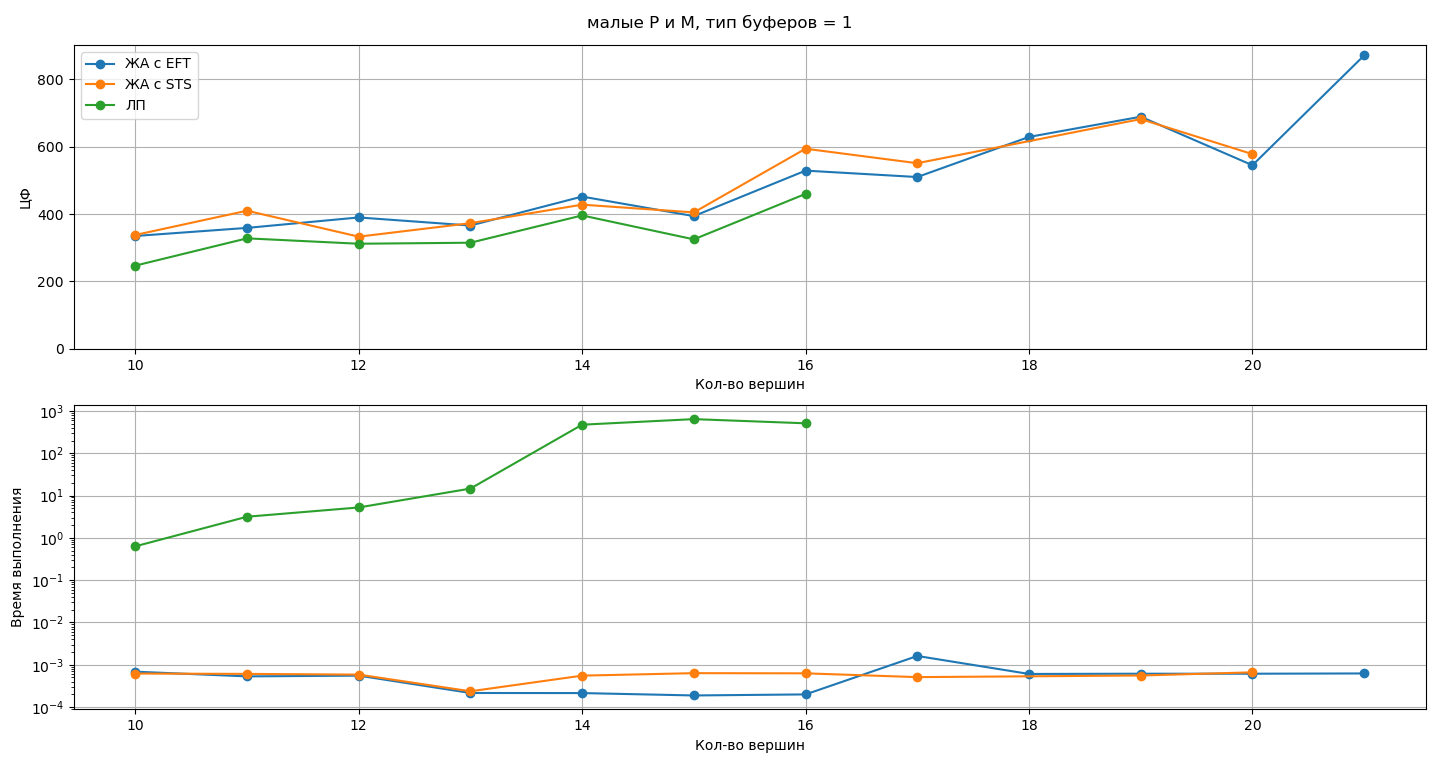
\includegraphics[width=1\textwidth]{pictures/low_P_and_M_1.png}
	\captionof{figure}{}
	\label{fig:scal1}
\end{center}

\begin{center}
	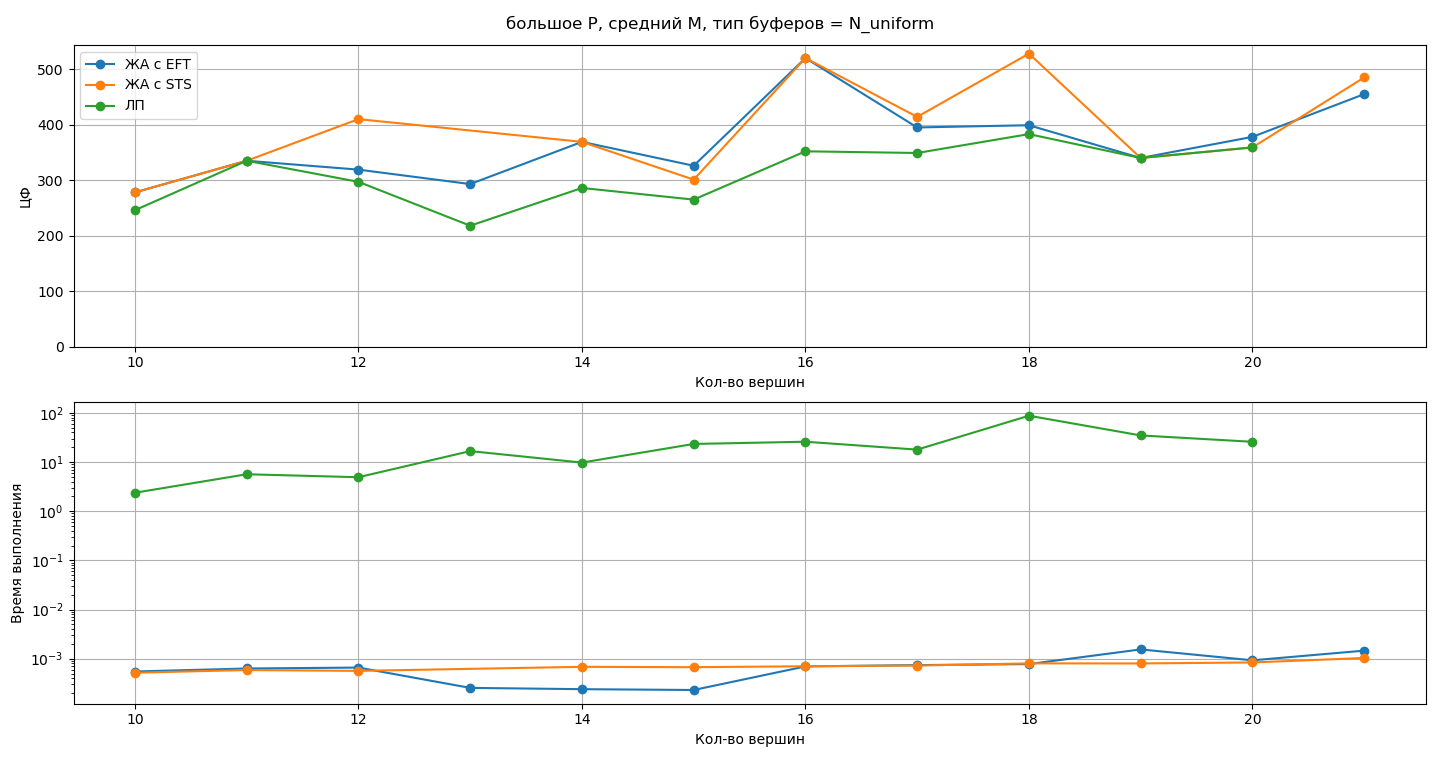
\includegraphics[width=1\textwidth]{pictures/high_P_mid_M_N_uni.png}
	\captionof{figure}{}
	\label{fig:scal4}
\end{center}

 На рисунке~\ref{fig:scal6} уже видно, что ЖА с STS не всегда завершается, в данном случае ему при любом числе процессоров не хватает минимального лимита памяти. На рисунке~\ref{fig:scal8} видно, как на графе с 15 вершинами уже долго работает ЛП при 2 доступных процессорах, но при этом всегда находит заметно лучшее расписание. На рисунке~\ref{fig:scal9} уже видно, что при 16 вершинах ЛП не завершается при P = 2. И на рисунке~\ref{fig:scal14} видно, как соотносятся алгоритмы на слоистом графе большого размера, видно, что там, где ЛП завершается, он часто дает заметно лучшее расписание по сравнению с ЖА. 

\begin{center}
	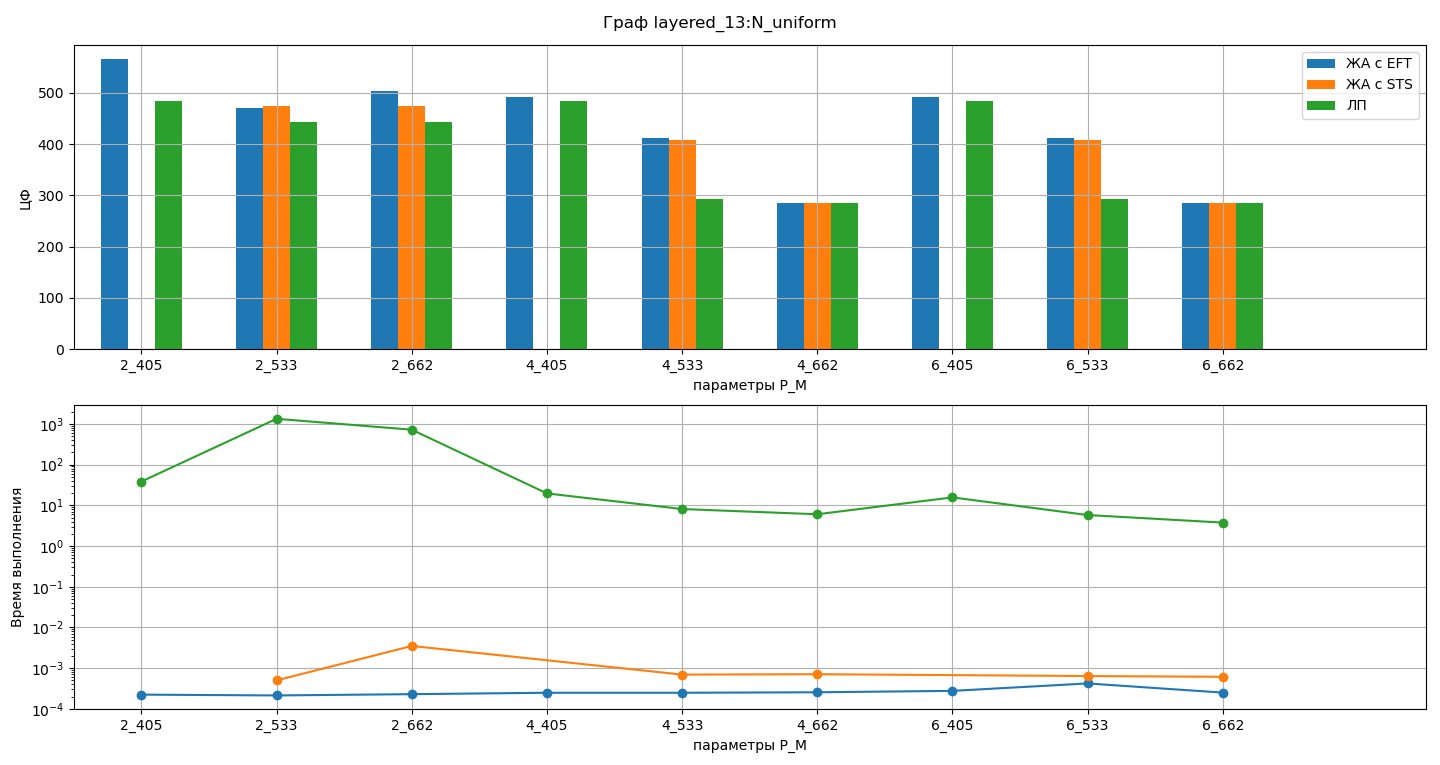
\includegraphics[width=1\textwidth]{pictures/layered_13_N_uni.png}
	\captionof{figure}{}
	\label{fig:scal6}
\end{center}

\begin{center}
	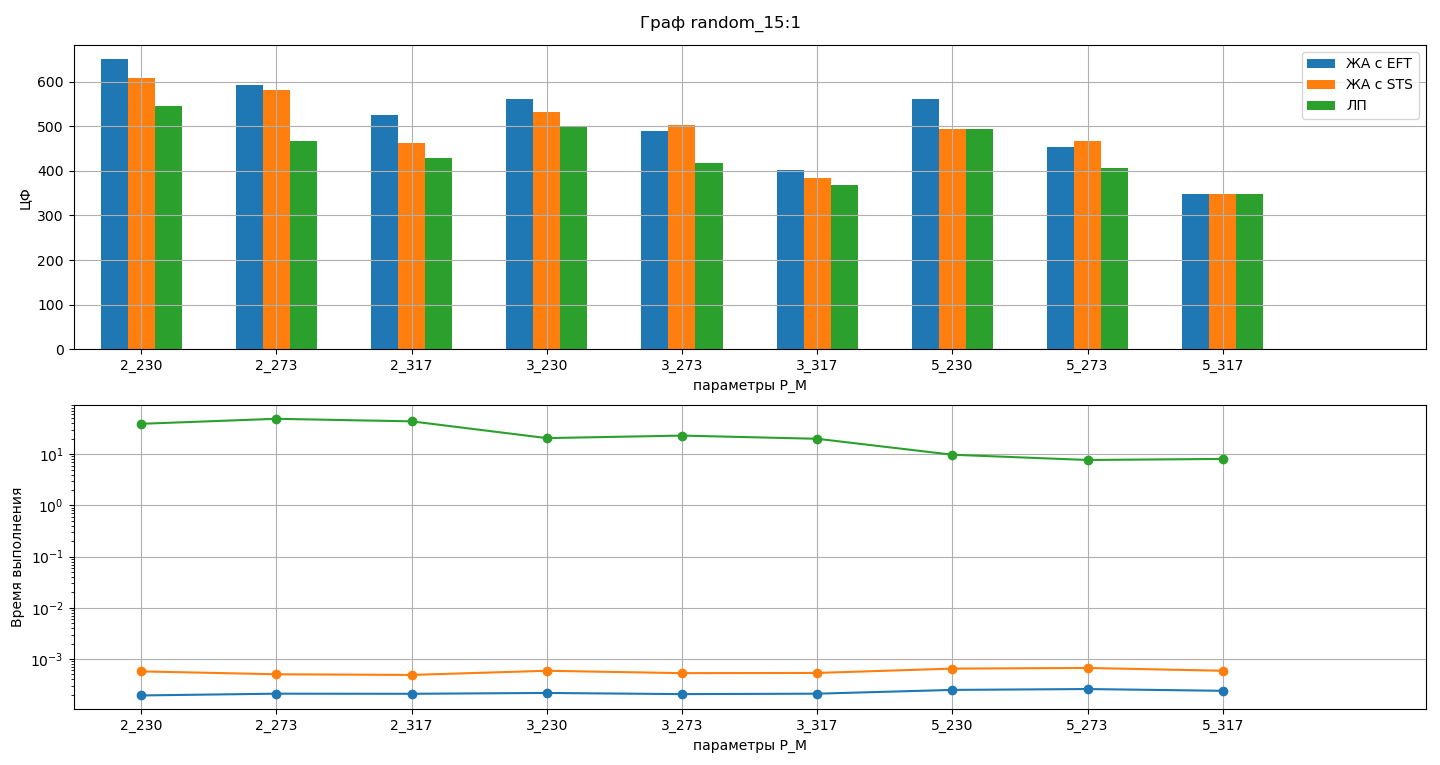
\includegraphics[width=1\textwidth]{pictures/random_15_1.png}
	\captionof{figure}{}
	\label{fig:scal7}
\end{center}

\begin{center}
	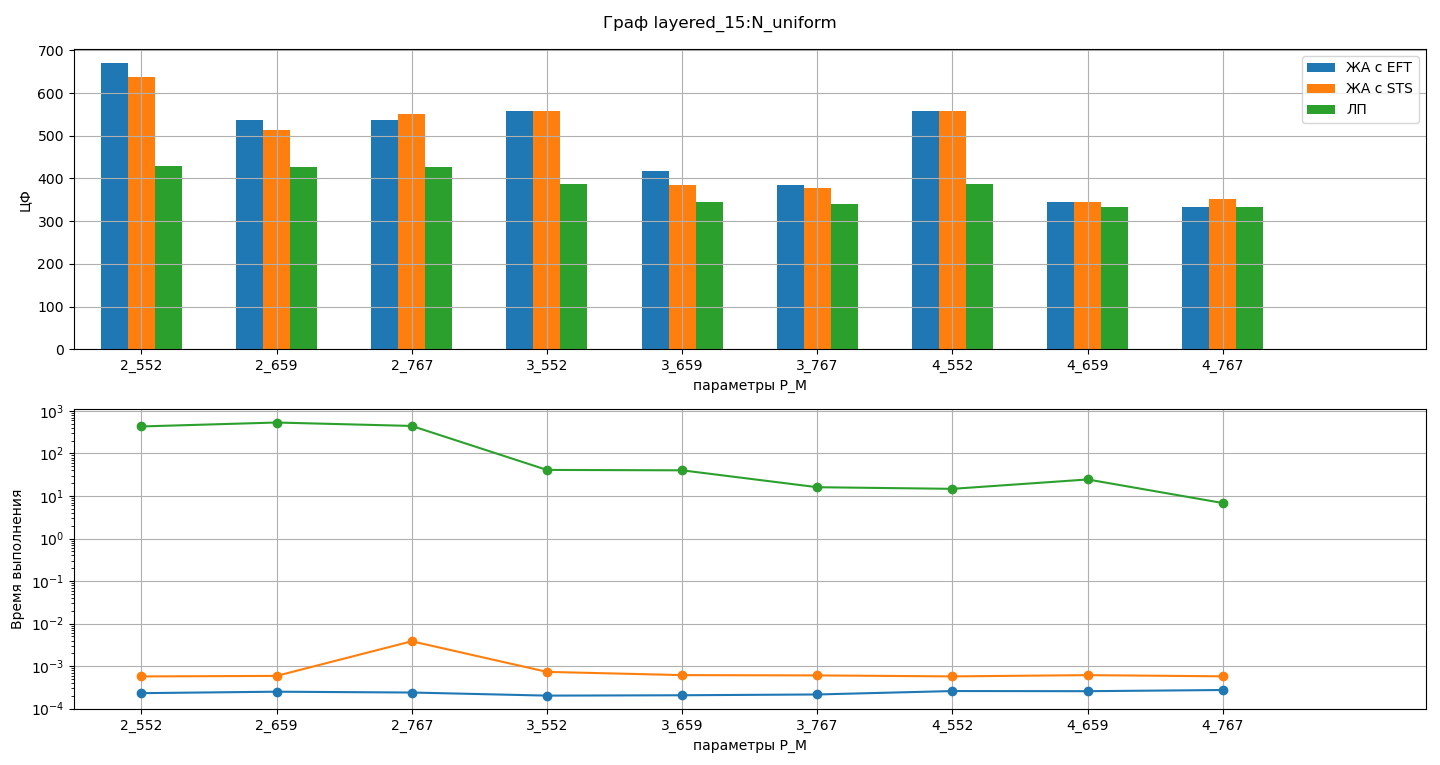
\includegraphics[width=1\textwidth]{pictures/layered_15_N_uni.png}
	\captionof{figure}{}
	\label{fig:scal8}
\end{center}

\begin{center}
	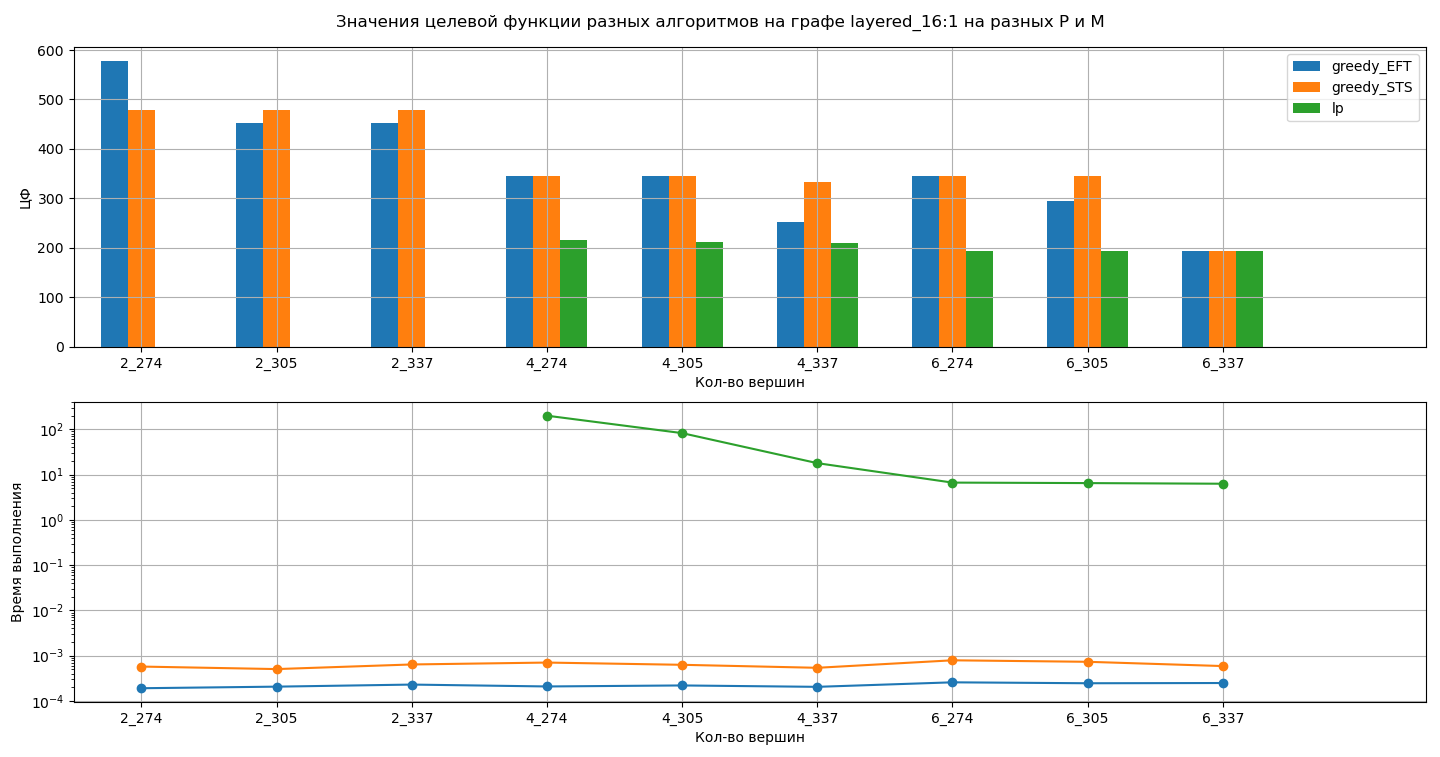
\includegraphics[width=1\textwidth]{pictures/layered_16_1.png}
	\captionof{figure}{}
	\label{fig:scal9}
\end{center}

\begin{center}
	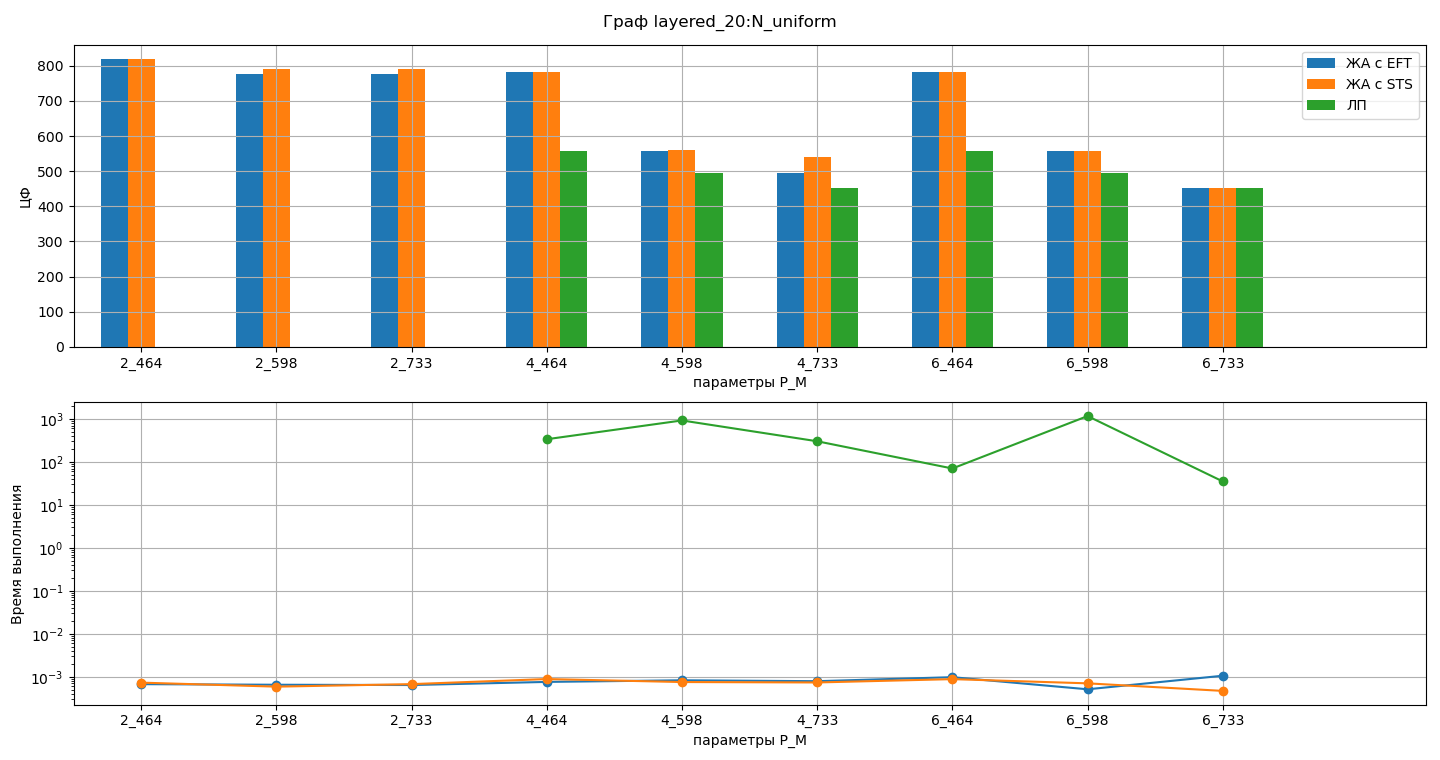
\includegraphics[width=1\textwidth]{pictures/layered_20_N_uni.png}
	\captionof{figure}{}
	\label{fig:scal14}
\end{center}


На рисунках~\ref{fig:EFT_12}-~\ref{fig:STS_12} видно, как ЖА с EFT может быть заметно лучше ЖА с STS, граф - layered\_12\_1\_2\_321. На рисунках~\ref{fig:EFT_16}-~\ref{fig:STS_16} видно обратную ситуацию, граф - layered\_16\_1\_2\_274. 

\begin{center}
	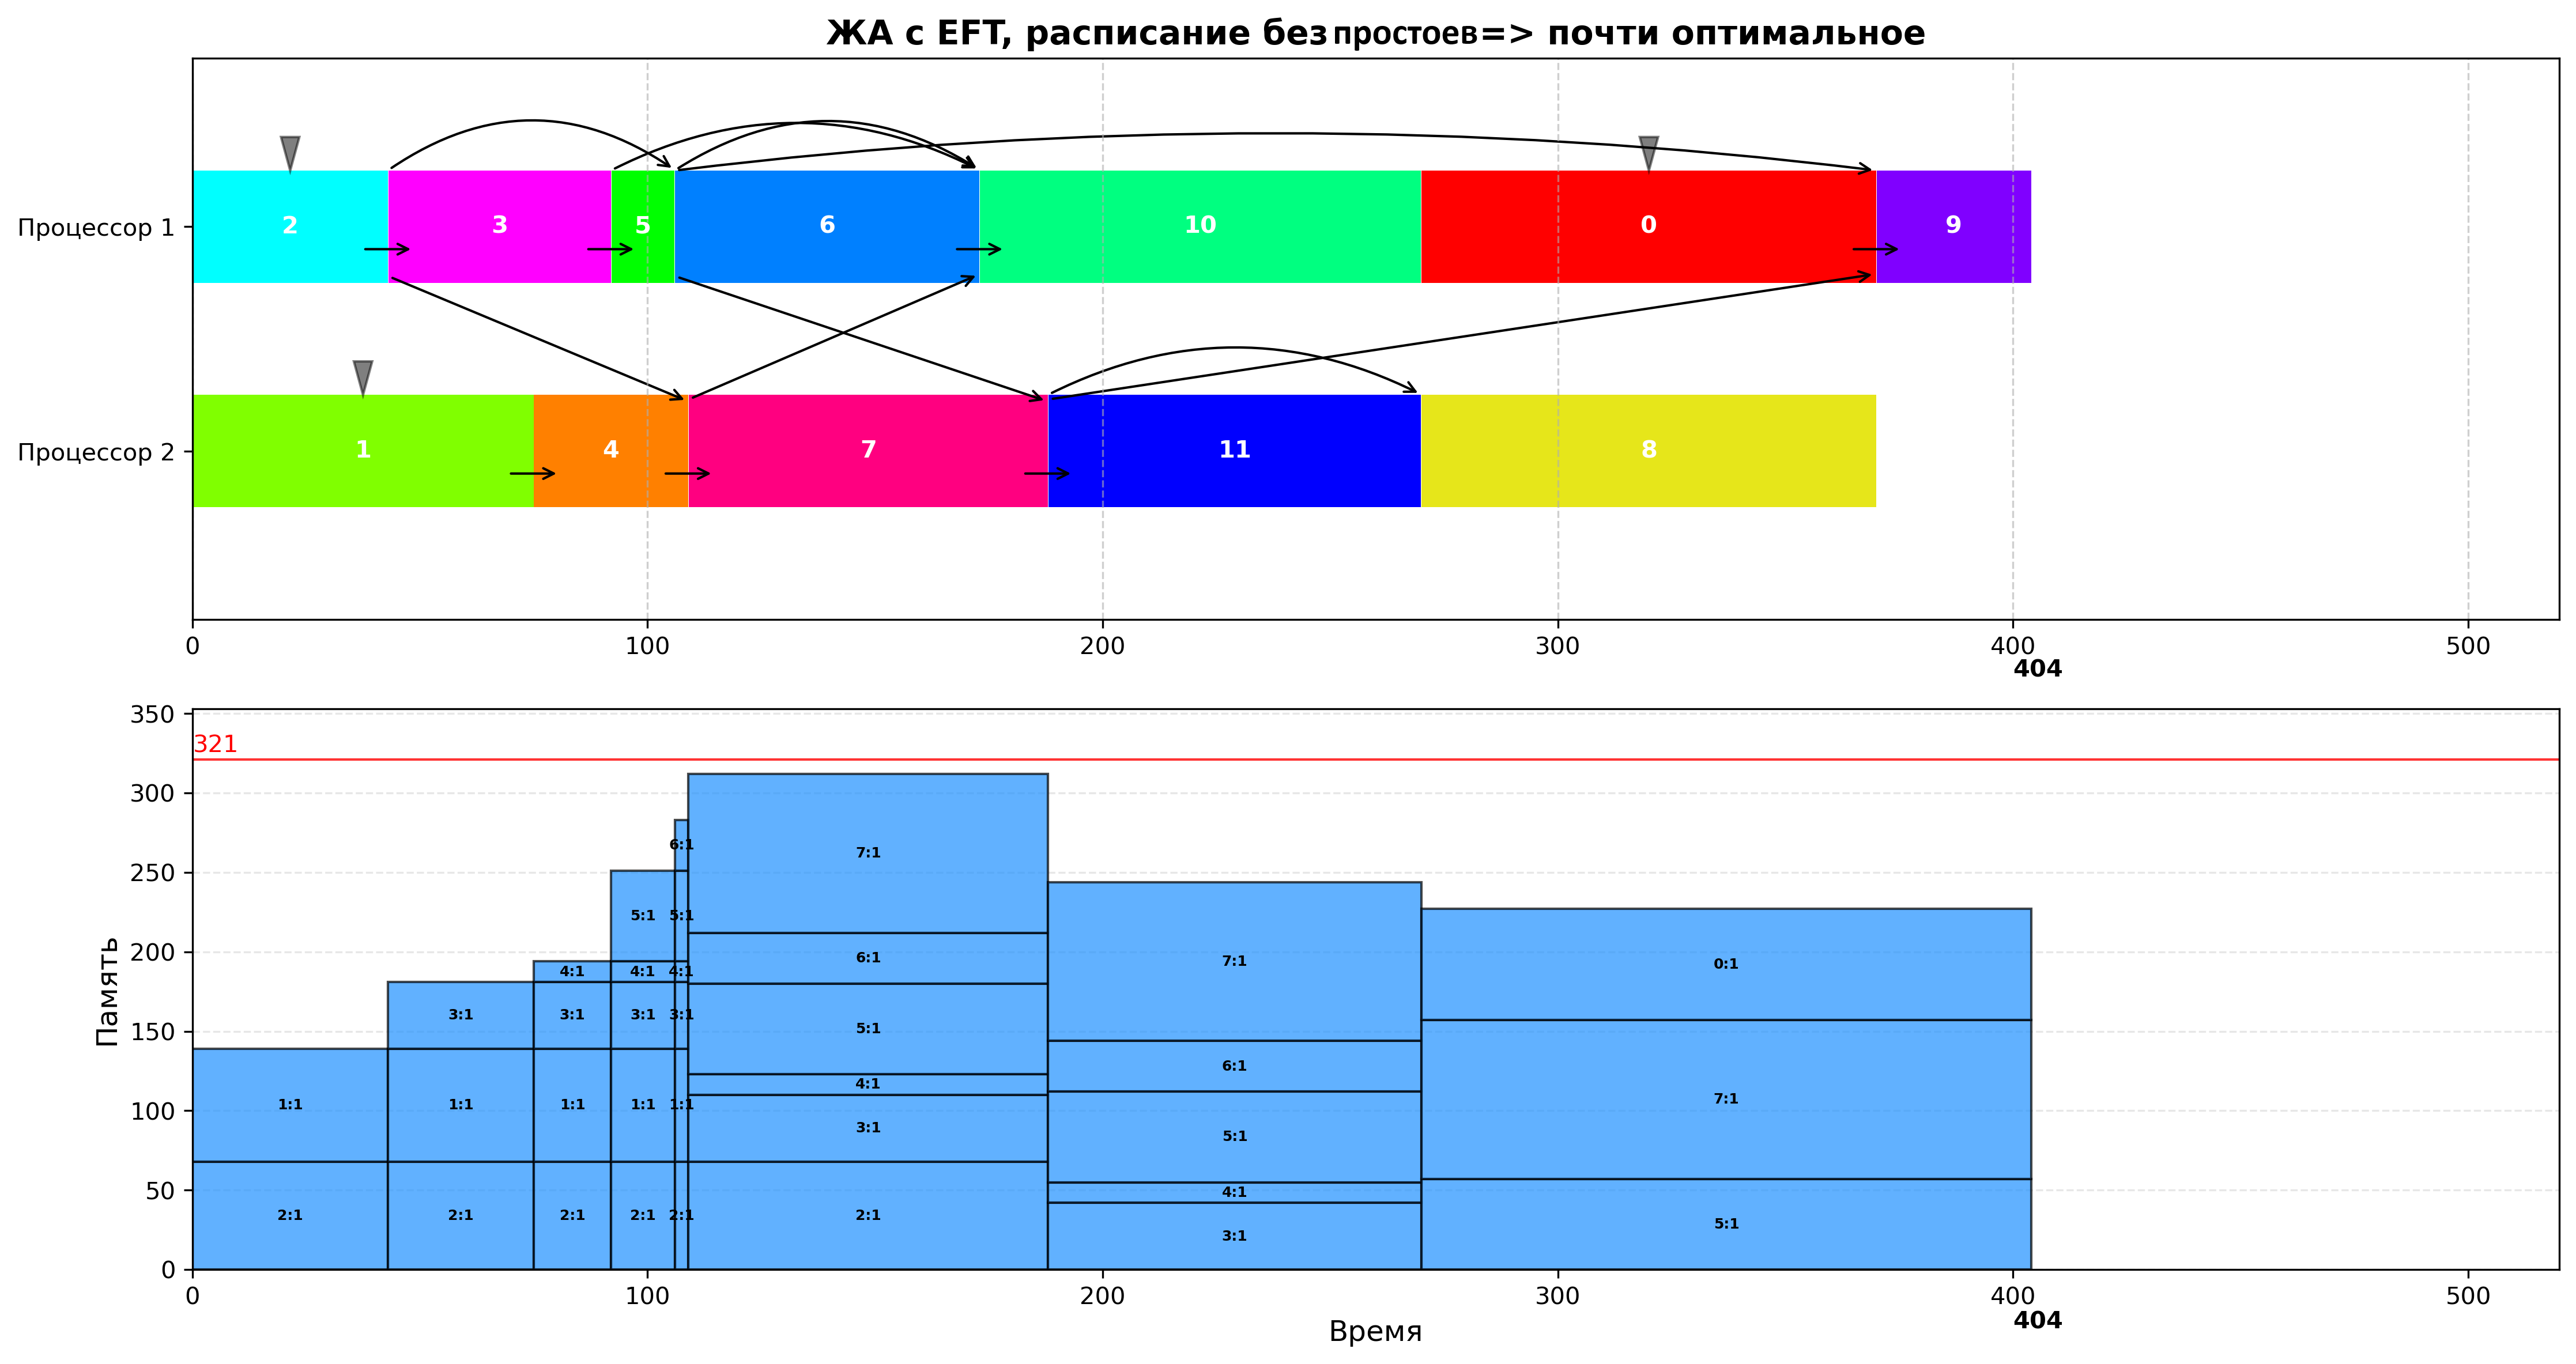
\includegraphics[width=0.8\textwidth]{pictures/greedy_EFT_layered_12_1_lp2_2_321.png}
	\captionof{figure}{}
	\label{fig:EFT_12}
\end{center}

\begin{center}
	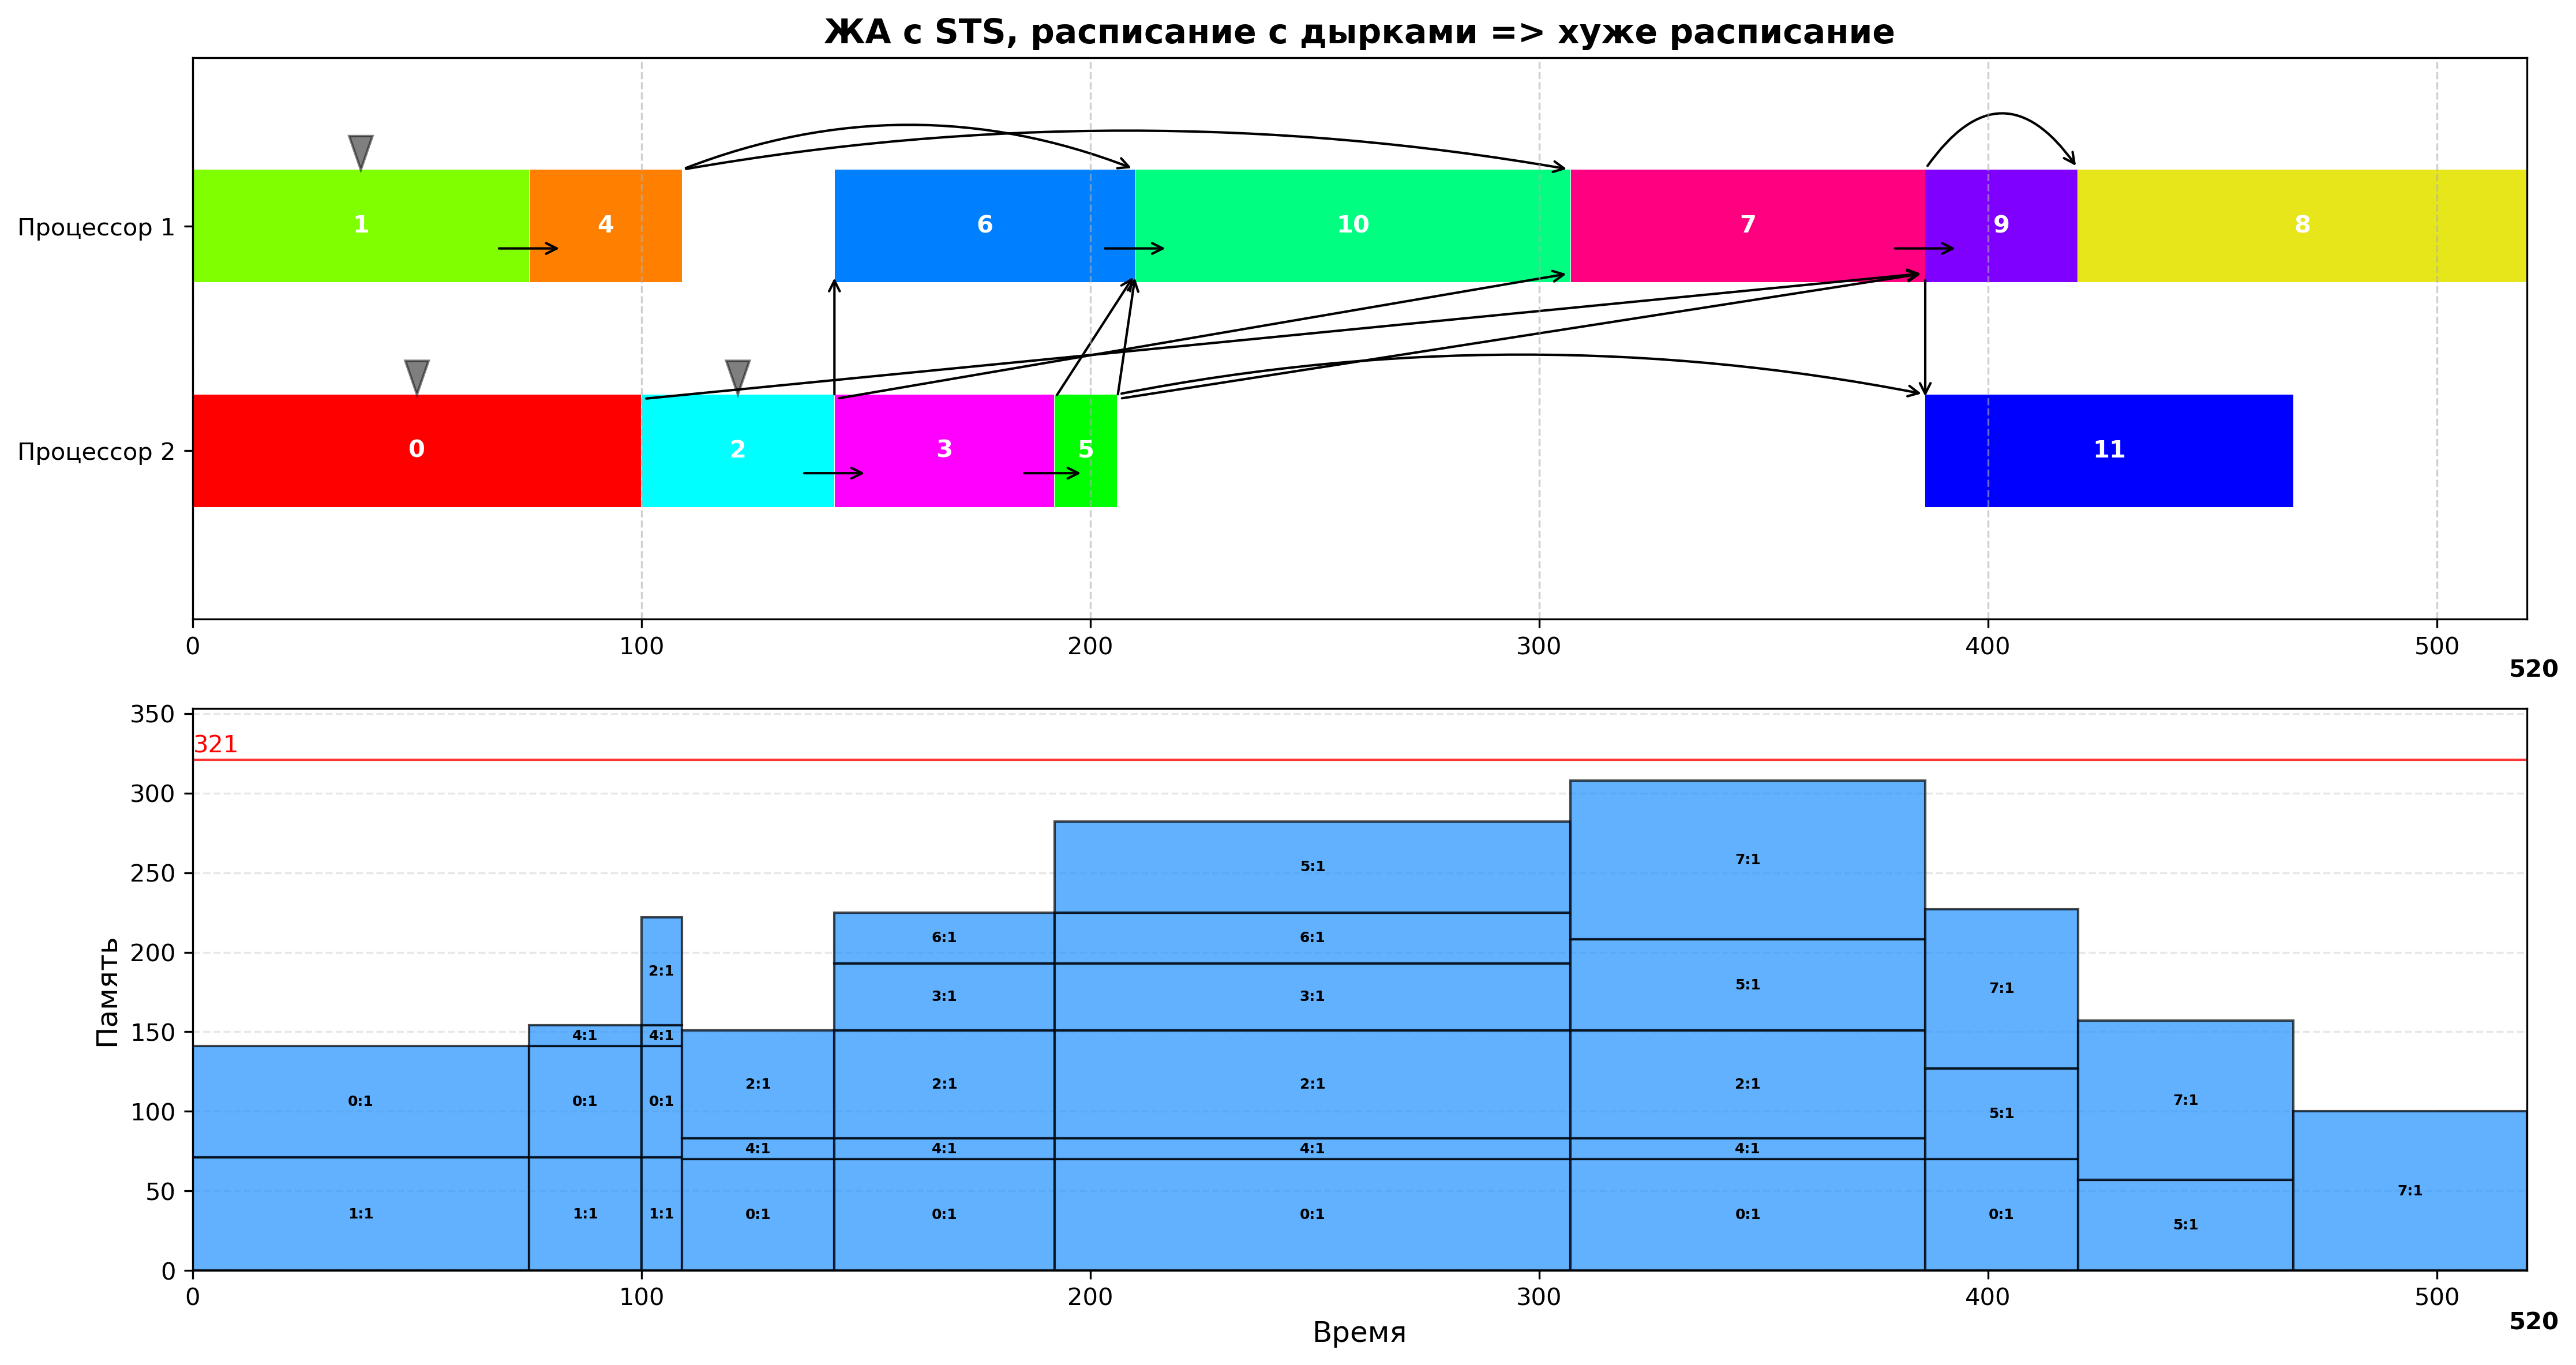
\includegraphics[width=0.8144\textwidth]{pictures/greedy_STS_layered_12_1_lp2_2_321.png}
	\captionof{figure}{}
	\label{fig:STS_12}
\end{center}

\begin{center}
	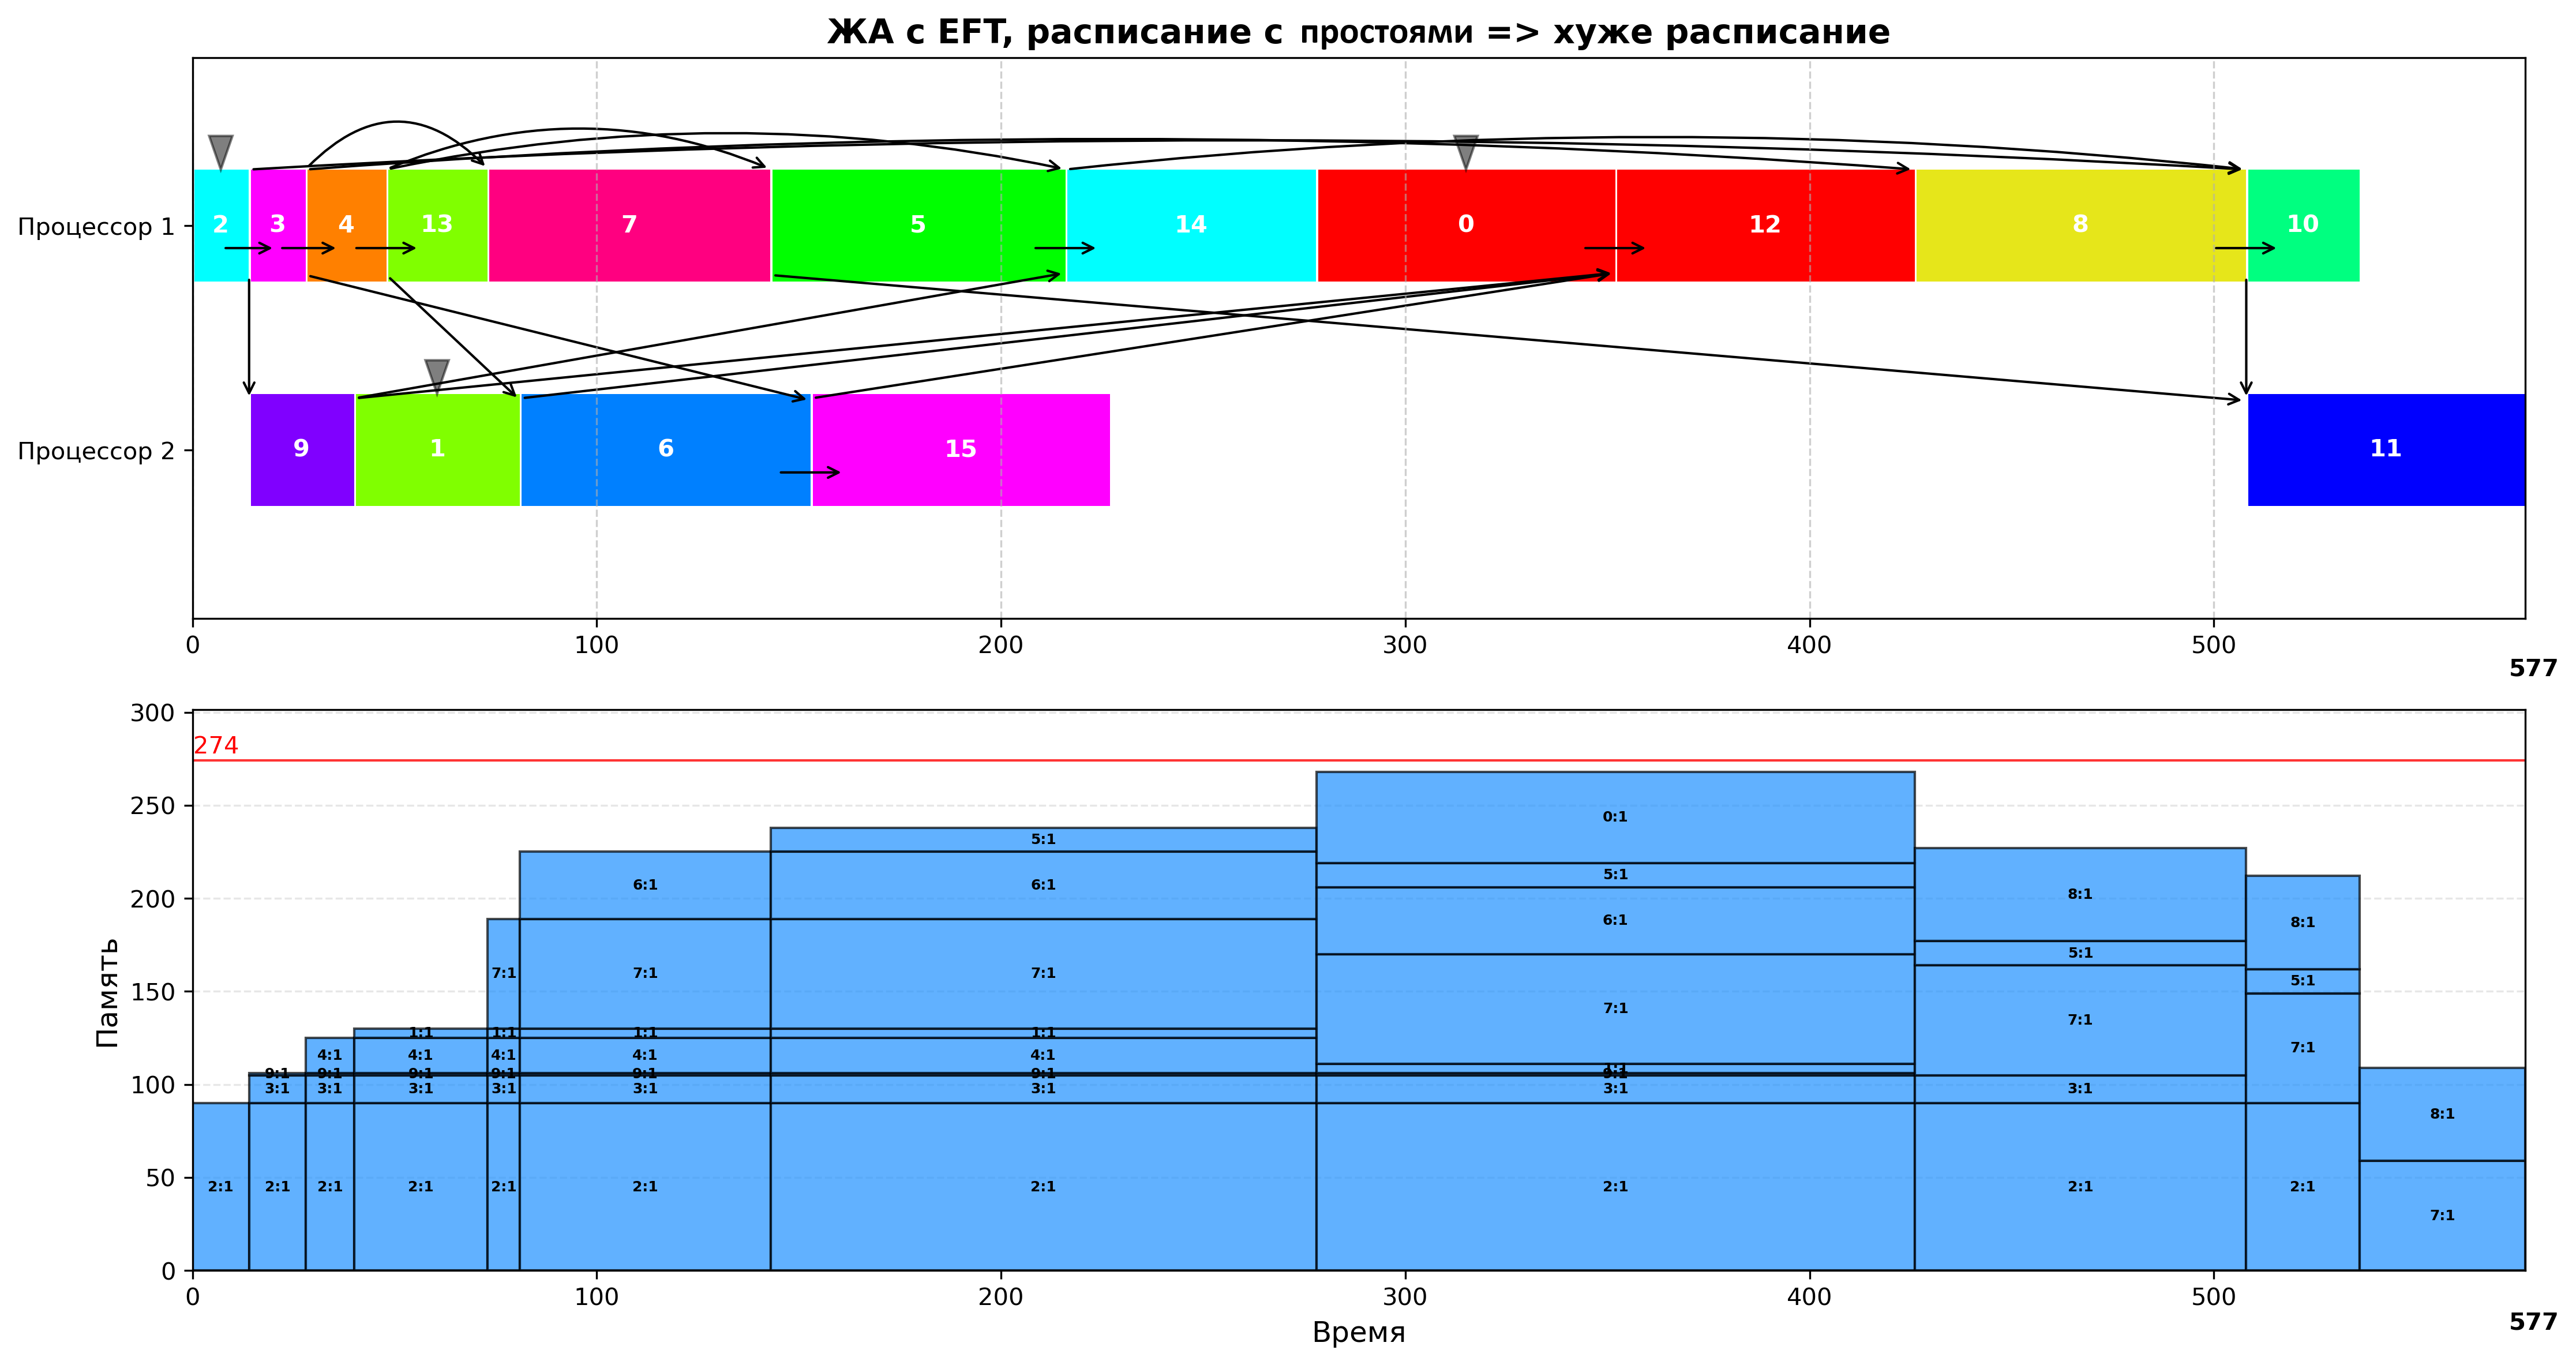
\includegraphics[width=1.018\textwidth]{pictures/greedy_EFT_layered_16_1_lp2_2_274.png}
	\captionof{figure}{}
	\label{fig:EFT_16}
\end{center}

\begin{center}
	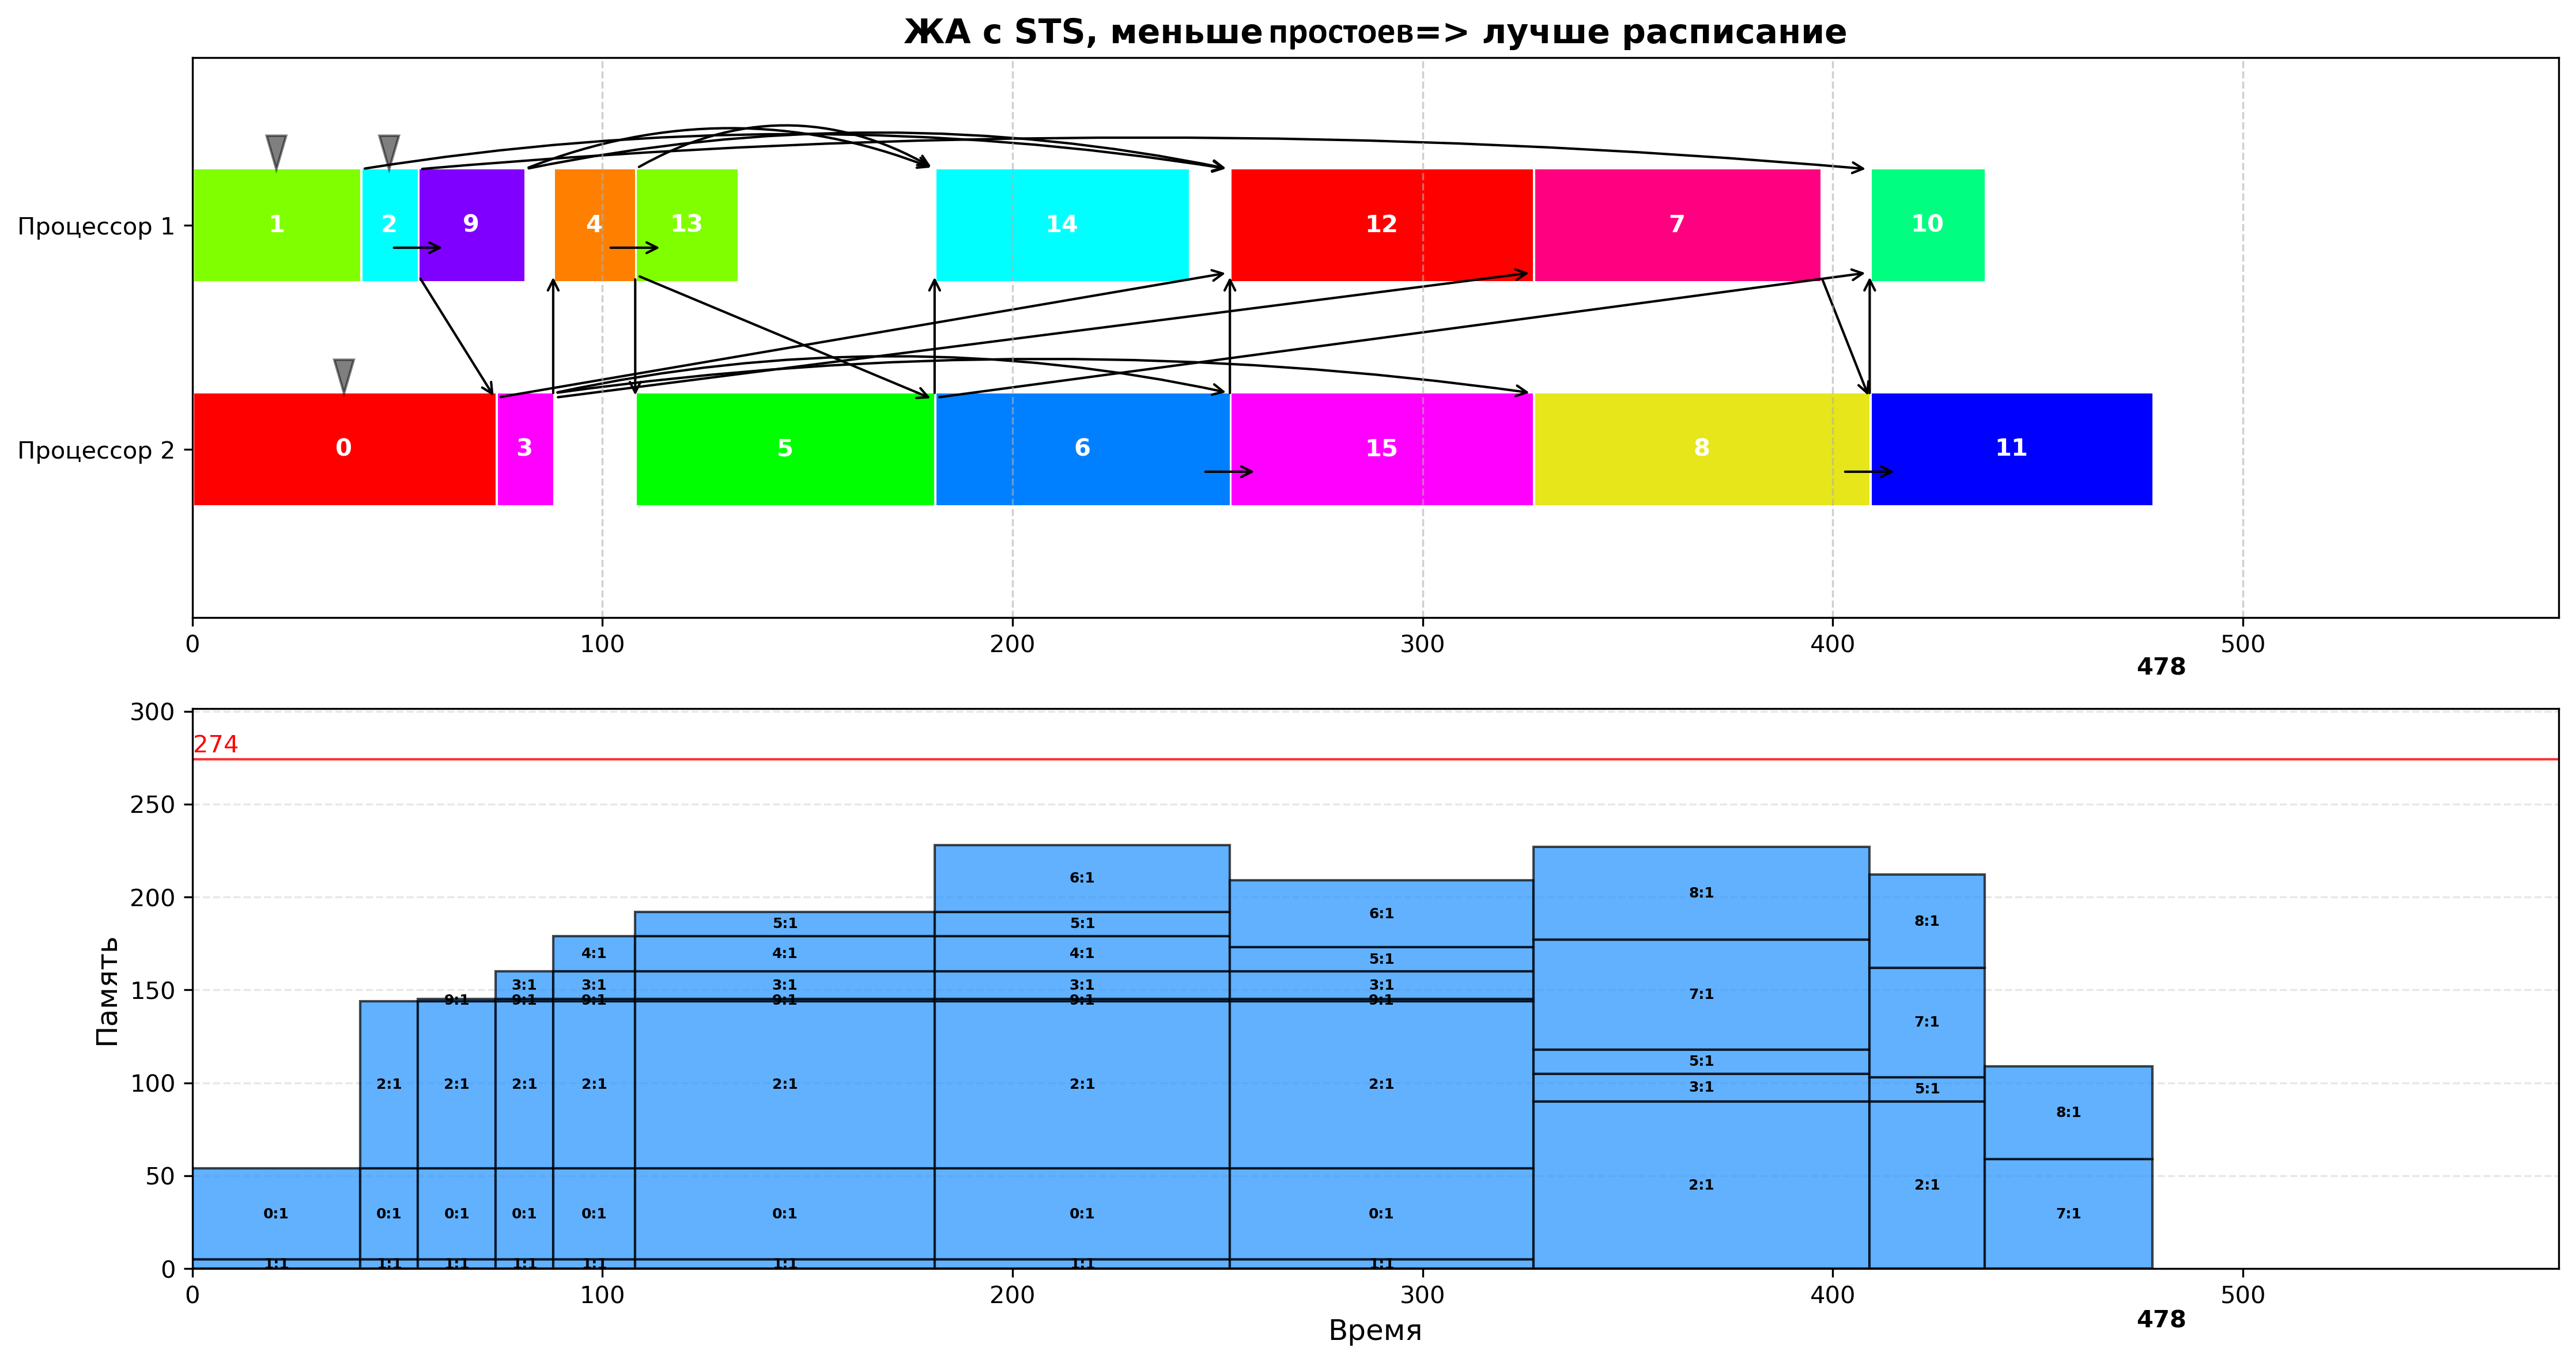
\includegraphics[width=1\textwidth]{pictures/greedy_STS_layered_16_1_lp2_2_274.png}
	\captionof{figure}{}
	\label{fig:STS_16}
\end{center}




\begin{center}
	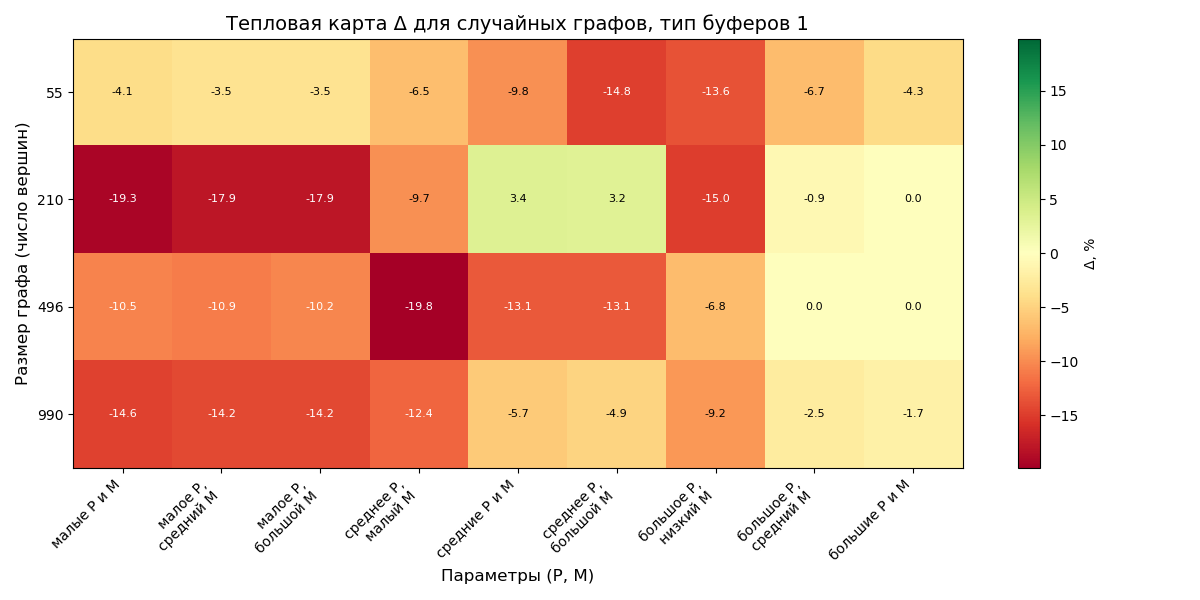
\includegraphics[width=1\textwidth]{pictures/heat_random_1.png}
	\captionof{figure}{}
	\label{fig:heat_rand}
\end{center}

\begin{center}
	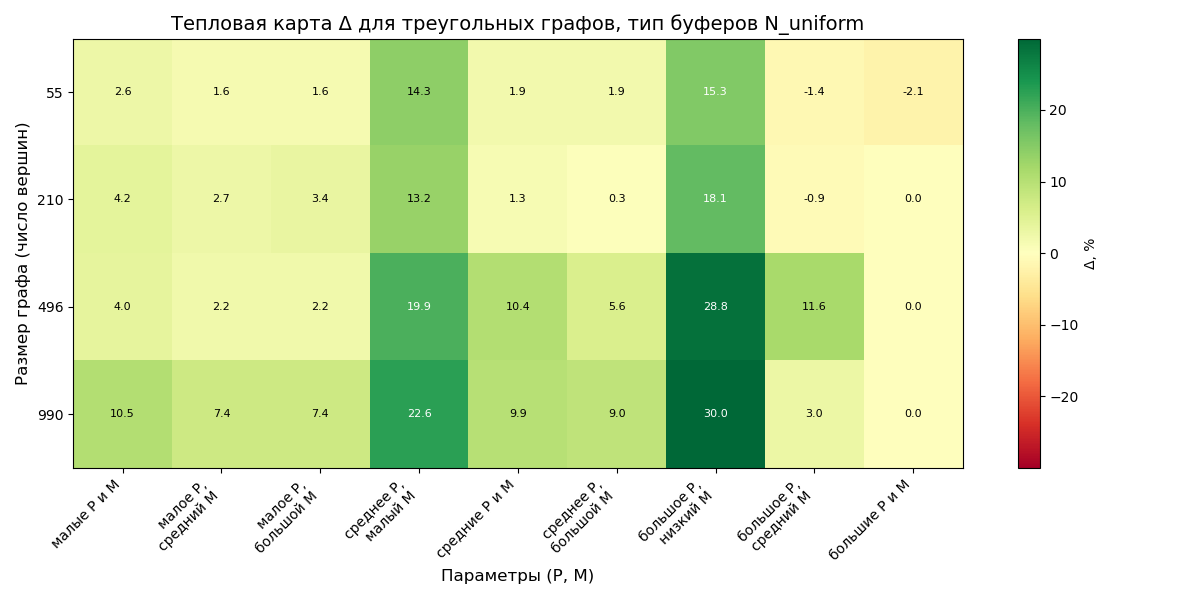
\includegraphics[width=1\textwidth]{pictures/heat_triadags_N_uni.png}
	\captionof{figure}{}
	\label{fig:heat_tri}
\end{center}
